% !TEX encoding = UTF-8 Unicode
% !TEX program = xelatex
\documentclass[10pt,aspectratio=169]{beamer}
\setbeamercovered{transparent=10}
\usetheme[purple,colorblocks]{Verona}
% 时间轴替换作者和标题所在的页脚区域，右侧保留页码。
% 删除 [subsections] 可改为按大章节显示；注释下一行可恢复原始页脚。
\useoutertheme[subsections]{sysutimeline}

\usepackage{xeCJK}
% 优先使用思源/Noto 中文字体；其他环境可回退到 TeX Live 自带的 Fandol。
\IfFontExistsTF{Noto Sans CJK SC}{%
  \setCJKmainfont{Noto Serif CJK SC}
  \setCJKsansfont{Noto Sans CJK SC}
  \setCJKmonofont{Noto Sans Mono CJK SC}
  \setCJKfamilyfont{zhli}{Noto Sans CJK SC}
}{%
  \setCJKmainfont{FandolSong-Regular.otf}[BoldFont=FandolSong-Bold.otf]
  \setCJKsansfont{FandolHei-Regular.otf}[BoldFont=FandolHei-Bold.otf]
  \setCJKmonofont{FandolFang-Regular.otf}
  \setCJKfamilyfont{zhli}{FandolHei-Regular.otf}[BoldFont=FandolHei-Bold.otf]
}
% 保留 Verona 主题的字体接口，中文版标题统一使用中文黑体。
\providecommand{\lishu}{\CJKfamily{zhli}}

\usepackage{tikz}
\usetikzlibrary{fadings}
\usepackage{listings}
\usepackage{caption}
\usepackage{subcaption}
\usefonttheme{professionalfonts}
\def\mathfamilydefault{\rmdefault}
\usepackage{amsmath}
\usepackage{multirow}
\usepackage{booktabs}
\usepackage{bm}
\definecolor{col}{RGB}{4,74,21}
\renewcommand{\figurename}{图}
\renewcommand{\tablename}{表}
\renewcommand{\lstlistingname}{代码}

\setbeamertemplate{section in toc}{\hspace*{1em}\inserttocsectionnumber.~\inserttocsection\par}
\setbeamertemplate{subsection in toc}{\hspace*{2em}\inserttocsectionnumber.\inserttocsubsectionnumber.~\inserttocsubsection\par}
\setbeamerfont{subsection in toc}{size=\small}
\AtBeginSection[]{%
  \begin{frame}{目录}
    \textbf{\tableofcontents[currentsection]}
  \end{frame}
}
\AtBeginSubsection[]{%
  \begin{frame}{目录}
    \textbf{\tableofcontents[currentsection,currentsubsection]}
  \end{frame}
}

\title{中山大学 Beamer 演示模板}
\subtitle{中文示例与页脚时间轴}
% 按需替换为实际汇报人的姓名、邮箱和单位。
\author[TY.Qi]{Tianyu Qilllll}
\mail{qitianyuqty@163.com}
\institute[中山大学]{网络空间安全学院\\中山大学}
\date{\number\year 年\number\month 月\number\day 日}
\titlegraphic[width=3cm]{sysu_logo}{}

\begin{document}

\maketitle

% 中文注释通过 escapeinside 交给 XeLaTeX 排版。
\defverbatim[colored]\lstI{%
  \begin{lstlisting}[language=C++,basicstyle=\ttfamily\small,
    keywordstyle=\color{structure.fg},escapeinside={(*@}{@*)}]
#include <iostream>

int main() {
    // (*@计算两个整数的和。@*)
    int a = 2;
    int b = 3;
    std::cout << a + b << std::endl;
    return 0;
}
  \end{lstlisting}
}

\section{基础示例}

\subsection{内容块}
\begin{frame}[c]{内容块}
  以下展示三种常用的内容块。
  \begin{block}{普通内容块}
    用于呈现基本概念、研究背景或一般说明。
  \end{block}
  \begin{exampleblock}{示例内容块}
    用于展示具体示例、实验步骤或应用场景。
  \end{exampleblock}
  \begin{alertblock}{强调内容块}
    用于突出关键结论、注意事项或重要问题。
  \end{alertblock}
\end{frame}

\subsection[列表与动画]{列表与逐步显示}
\begin{frame}[c]{列表与逐步显示}

  {\large 有序列表示例}
  \begin{enumerate}[<+->]
    \item 第一项内容
    \item 第二项内容
    \item 第三项内容
  \end{enumerate}
  \vfill
  {\large 无序列表示例}
  \begin{itemize}[<+->]
    \item 第一项内容
    \item 第二项内容
    \item 第三项内容
  \end{itemize}
\end{frame}

\subsection{双栏排版}
\begin{frame}[c]{双栏排版}
  \begin{columns}[onlytextwidth]
    \column{0.4\textwidth}
      左栏：质能关系式
      \begin{equation}
        E = mc^2
      \end{equation}
    \column{0.4\textwidth}
      右栏：牛顿第二定律
      \begin{equation}
        F = ma
      \end{equation}
  \end{columns}
\end{frame}

\subsection[图形与代码]{图形与代码展示}
\begin{frame}[c]{图形展示}
  \begin{figure}
    \centering
    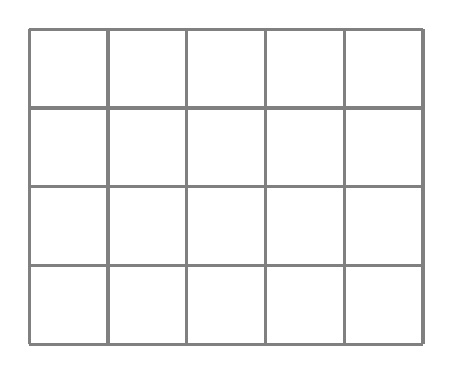
\begin{tikzpicture}
      \draw[help lines,very thick] (0,0) grid (5,4);
    \end{tikzpicture}
    \caption{使用 Ti\textit{k}Z 绘制的网格示例}
  \end{figure}
\end{frame}

\begin{frame}{代码展示}{C++ 示例}
  \lstI
\end{frame}

% 致谢页采用 plain 样式，自动隐藏时间轴与页码。
\beamertemplateshadingbackground{structure.fg!90}{structure.fg}
\begin{frame}[plain]
  \vfill
  \centering
  {\Huge\color{white} 感谢聆听！\\[10pt]欢迎提问与交流}
  \vfill
\end{frame}

\end{document}
